\section{Application}\label{sec:application}
The following section will describe the implemented and applied techniques and model architectures, will display results of the experiments done here, describe the validation process of the final architectures and give a brief introduction about the roadblocks that were faced while implementing the experiments.

\subsection{Chosen Model Architectures}\label{subsec:model-architectures}
To solve the tasks of classification and Bounding Box regression individually and combined several methods were chosen to train and compare in benchmark tests.
\subsubsection{Conventional Methods}
All experiments for conventional methods were performed on PCA-reduced data sets, as described in "\nameref{subsec:dimensionality-reduction}", for this purpose the data set gets transformed onto the first $100$ and $400$ PCs of the training set.\\
\textbf{Ridge Regression}\\
The Ridge Regression model as introduced in "\nameref{subsec:linear-regression}" is a single output predictor.
To convert it to a multi-output Ridge Regression the implementation of \path{MultiOutputRegressor}~\footnote{scikit-learn overview of multiclass and multioutput algorithms: \url{https://scikit-learn.org/stable/modules/multiclass.html}} was used.
\path{RidgeReg1} the first model that gets as input images transformed onto the $100$ first PCs and \path{RidgeReg2} the second model using $400$ first PCs of the regression data set that yields elements of shape \eqref{eq:regression-sample} accordingly.\\
\textbf{SVMs}\\
For the classification task conventional linear SVMs were applied.
Unlike the RidgeReg model, SVMs as implemented in footnote 28 can be applied for multi-class classification tasks directly without an additional wrapper method.
Again, 100 (\path{SVM_1}) and 400 (\path{SVM_2}) extracted PCs of the cropped data set \eqref{eq:classification-sample} have been used to solve the classification task.
\subsubsection{CNN-Backbones}
As stated in \nameref{subsec:cnn} the here implemented CNN-architectures are purely used for the task of extracting features from images, so called Backbones.
Additional to these Backbones a dedicated "\nameref{subsubsec:task-solving-head}" was added according to the underlying training strategy.
The architecture of the task solving heads will be described in the upcoming sub-section.\\
\textbf{INet}\\
$INet$ is a custom CNN architecture implemented.
Several iterations of experiments using different approaches led to the architecture used in this paper, a graph of the architecture can be found in \figref{fig:inet}.
The parameters used to create this architecture were selected according to best practices in the field, such as the pyramid structured conv. layers, but are also part of initial experiments while searching for an architecture.
\newline
\textbf{State of the Art (SotA) Architectures}\\
As discussed, this paper compares the results from previously mentioned methods, to state of the art architectures \textit{VGG-16}, \textit{MobileNet} and \textit{YOLO}.
Whereas VGG and MobileNet are \textit{classical} CNN architecture, YOLO differs in many aspects.
Explaining each of the architectures in detail will go beyond the scope of this paper.
To get a full overview and read more about the details in the implementations of these architectures,
t reader is encouraged to look into the papers~\cite{VGG16, MobileNet, yolo}, as well as looking into surveys~\cite{Jiao_2019} that have been published over the last years, or the \href{https://github.com/tensorflow/models}{Tensorflow "models" project}.
The implementations of VGG-16 and MobileNet applied here are part of the \path{keras}\footnote{\url{https://keras.io/}} library and can be imported easily. Both models were used with pretrained weights. Those weights have been trained on the \path{'imagenet'} data set.
For the YOLO architecture the YOLOv5~\footnote{
    YOLOv5 github source: \url{https://github.com/ultralytics/yolov5}
} was applied.
\begin{figure}[!ht]
    \centering

    \begin{tikzpicture}

    \node (X) at (0,0) {\small$X$};

    \node[bn,rotate=90,minimum width=3.5cm] (bn) at (1.25,0) {\small BN};
    \node[conv,rotate=90,minimum width=3.5cm] (conv1) at (2.75,0) {\small$\text{conv-block}_{16, 3, 3}$};
    \node[conv,rotate=90,minimum width=3.5cm] (conv2) at (4.25,0) {\small$\text{conv-block}_{32, 3, 3}$};
    \node[conv,rotate=90,minimum width=3.5cm] (conv3) at (5.75,0) {\small$\text{conv-block}_{64, 3, 3}$};
    \node[conv,rotate=90,minimum width=3.5cm] (conv4) at (7.25,0) {\small$\text{conv-block}_{128, 3, 3}$};
    \node[conv,rotate=90,minimum width=3.5cm] (conv5) at (8.75,0) {\small$\text{conv-block}_{256, 3, 3}$};

    \node (f) at (10.5,0) {\small Features};


    \draw[->] (X) -- (bn);
    \draw[->] (bn) -- (conv1);
    \draw[->] (conv1) -- (conv2);

    \draw[->] (conv2) -- (conv3);

    \draw[->] (conv3) -- (conv4);

    \draw[->] (conv4) -- (conv5);
    \draw[->] (conv5) -- (f);
    \end{tikzpicture}
    \caption{CNN Backbone feature extractor architecture. The input gets normalized using batch normalization, then gets processed by a series of convolutional blocks. Each of the blocks consists of a conv-layer\footnotemark, BN, $\ReLU$ and global-$\max$-pooling layer and is using $3\times 3$-filter masks. The $i$-th  $\text{conv-block}_i$ has $2^{4+i}$ filter masks, for $i=0,\ldots,4$.}
    \label{fig:inet}
\end{figure}
\footnotetext{conv-layer: Convolutional Layer with activation function $\ReLU$ and parameters $n,h,w$ for number, height and width of the underlying filter masks.}
\subsubsection{Task-solving-Head}\label{subsubsec:task-solving-head}
To solve tasks based on extracted features the Backbone models from the previous section were extended by task solving heads.
For the purpose of this paper a global-max-pooling layer was added right after the feature extractor, then a Dropout layer with factor $0.5$, followed by a fully connected dense layer with $128$ neurons and ending with a dense block with the number of output neurons that the task requires.
The classification-Head consists of $K=5$ output neurons and for regression $K=4$, according to the descriptions in "\nameref{subsec:tasks}".
For the purpose of this paper a variety of different head architectures were explored until a satisfying combination of parameters was found.
A visualization including the parameters can be seen in \figref{fig:heads}.
The regularization factor $\alpha$ of the output dense-block is part of the HPO.

\begin{figure}[!ht]
    \centering
    \begin{tikzpicture}

    \node (f) at (0,0) {\small Features};
    \node[pool,rotate=90,minimum width=4.5cm] (pooling) at (2, 0) {\small$\text{global}-\max-\text{pool}$};
    \node[dropout,rotate=90,minimum width=4.5cm] (dropout) at (3.5, 0) {\small$\text{dropout}_{0.5}$};
    \node[fc,rotate=90,minimum width=4.5cm] (denseFull) at (5, 0) {\small$\text{dense}_{128}$};
    \node[denseBlock,rotate=90,minimum width=4.5cm] (denseBlock) at (6.5, 0) {\small$\text{BN}+\ReLU+\text{ dense}_{N,\alpha}$};
    \node (y) at (8,0) {\small $\mybold{\hat{y}}$ or $\mybold{\hat{c}}$};
    \draw[->] (f) -- (pooling);
    \draw[->] (pooling) -- (dropout);
    \draw[->] (dropout) -- (denseFull);
    \draw[->] (denseFull) -- (denseBlock);
    \draw[->] (denseBlock) -- (y);
    \end{tikzpicture}
    \caption{Visualization of task solving head. From left to right: Features get passed into a global max pooling layer, followed by a dropout layer with factor $0.5$. Then the reduced feature set gets passed into a fully-conntected dense layer with $128$ neurons. After the dense layer a final a dense block with  $N$ neurons and the regularization factor $\alpha$ calculates the final prediction.}
    \label{fig:heads}
\end{figure}
\subsection{Training results}\label{subsec:training-results}
For the experiments a small set of different feature extractors were trained and optimized using the Gaussian-Optimization as described in "\nameref{subsubsec:hpo}".
Each of the experiments was executed one the original data sets as described in "\nameref{subsec:datasets}", and an augmented version of them.
The HPs were selected according to \tabref{fig:reg-hp-table} and \tabref{fig:clf-hp-table}.
To compare the training results for the classification task the measures of Accuracy \eqref{eq:accuracy} and F1 \eqref{eq:f1} were selected.
For the regression task $\GIoU$ and $\RMSE$.
This and the following sections describe the most promising results, a full overview of all training results, including plots of loss function progressions, or the used HPs and their final sets, can be found in the code repository wiki~\footnote{Results listed at \url{https://gitlab.com/kinsecta/ml/thesisphilipp/-/wikis/home}, allows looking at results individually.}.
Here discussed results in combination with visualizations can be found in the "\nameref{sec:appendix}" section at the end of the document.\\
All architectures, except YOLOv5~\footnote{YOLOv5 is implemented in pytorch and requires a TF version \path{>= 2.4}. Therefore the YOLO model was trained on Google Colab using a GPU runtime environment (\url{https://colab.research.google.com/}).} have been trained on a dedicated server, provided by BHT, using a "NVIDIA Quadro RTX 8000" GPU, if not explicitly marked differently.

\subsubsection{Terminology}
The following sections will display assembled methods, also called solvers, and the results of training and validation experiments of these methods.\\
While describing these results three terms are used that will be summarized here briefly.
\begin{itemize}
    \item 2-stage-method: A solver, using two of the methods described in "\nameref{sec:machine-learning-methods}".
    \begin{itemize}
        \item Independent: This solver performs classification predictions on full images independently from the BB predictions.
        \item Sequential: This solver performs classification predictions on cropped images based on BB predictions from the applied regressor.
    \end{itemize}
    \item 1-stage-method: A solver, predicting both label types simultaneously based on full images.
\end{itemize}

\subsubsection{Conventional Methods}
Initially the conventional methods LinReg and SVM were fitted onto the individual training sets with samples in form \eqref{eq:regression-sample} and \eqref{eq:classification-sample} using a OvR method.
\begin{table}[!ht]
    \centering
    \begin{tabular}{|l|c|c|c|c|}
        \hline
        \textbf{Method} & \textbf{GIoU} & \textbf{RMSE}  & \textbf{Accuracy} & \textbf{F1} \\
        \hline
        \hline
        \multicolumn{5}{|l|}{\textit{PCA${}_{100}$} }
        \\
        \hline
        Ind. & $0.3481$ & $21.2985$ &$0.4806$ & $0.4725$\\
        Seq. & $0.3481$ & $21.2985$ & $0.284$ & $0.2685$ \\
        \hline
        \hline
        \multicolumn{5}{|l|}{\textit{PCA${}_{400}$} }
        \\
        \hline
        \textbf{Ind.} & $\mybold{0.3525}$ & $\mybold{20.9326}$ &$\mybold{0.5339}$ & $\mybold{0.5200}$\\
        Seq. & $0.3525$ & $20.9326$ & $0.3040$ & $0.2704$ \\
        \hline
    \end{tabular}
    \caption{Training results on the raw validation set for conventional methods fitted independently (Ind.), using the training set with shapes \eqref{eq:regression-sample} and \eqref{eq:cropped-sample}, and sequentially (Seq.), using the training set with shapes \eqref{eq:cropped-sample} based on the predictions done with the LinReg model. One set of methods was fitted using the reduction method $\text{PCA}_{100}$, the other $PCA_{400}$ as described in "\nameref{subsec:dimensionality-reduction}"\footnotemark.
    }
    \label{fig:conventional-results}
\end{table}
\footnotetext{Note that for the regression task the results are equal for the Independent and the Sequential Two-Stage-Strategies.}\\
Looking at the results presented in \tabref{fig:conventional-results} reveals that the conventional methods seem to generalize fine on the training data for the regression task.
The results for classification are mediocre to bad.
Once connected in the sequential (Seq.) approach the metrics for classification drop even more to a low of $30\%$ accuracy.
Another interesting learning is the comparison between the results obtained using $\text{PCA}_{100}$ and those using $\text{PCA}_{400}$.
Visualizations of predictions can be found in \figref{fig:conventional-predictions}, confusion matrices for visual validation are available in \figref{fig:conventional-confusions}.
In these plots it becomes more obvious how bad the classification predictions are.
As introduced in "\nameref{subsec:metrics}" the confusion matrix is desired to contain $1.0$ on its diagonal, here it is more like a random distribution.
These visualisations match the results of the metrics as listed in \tabref{fig:conventional-results}.

\begin{figure}[!ht]
    \centering
    \begin{minipage}{.45\textwidth}
    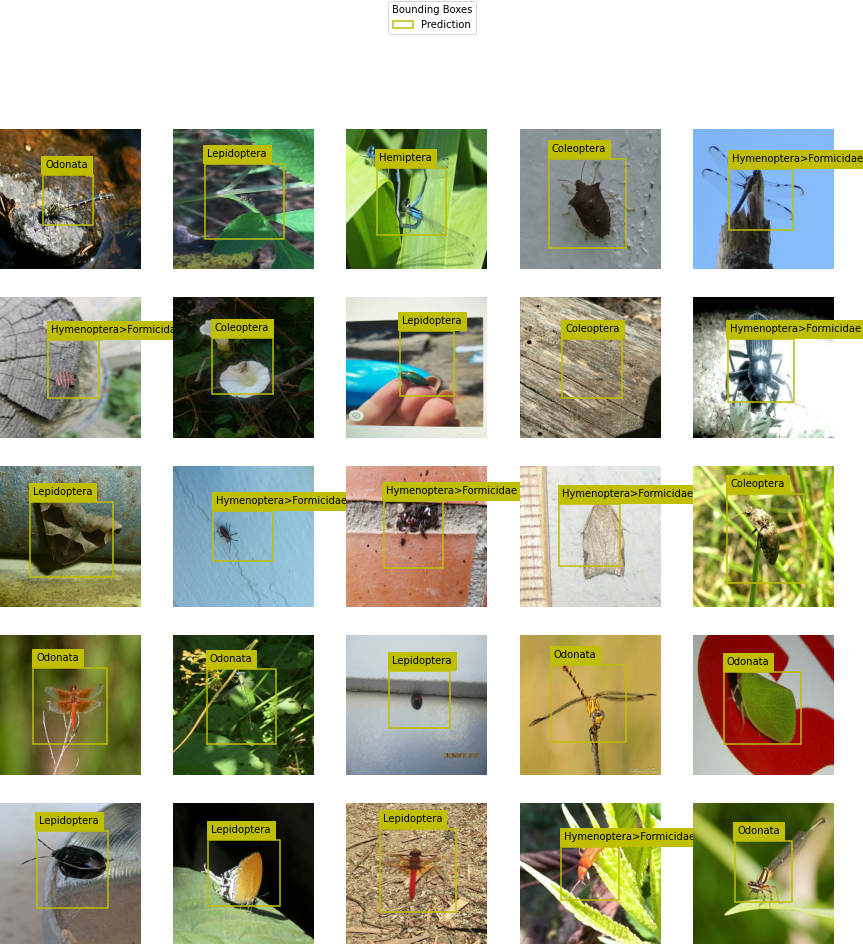
\includegraphics[width=\textwidth]{src/images/pca-ridge-svm-two-stage-model-predictions.png}
    \end{minipage}
    \hfill
    \begin{minipage}{.45\textwidth}
    \includegraphics[width=\textwidth]{src/images/pca-400-ridge-svm-two-stage-model-predictions.png}
    \end{minipage}
    \caption{Sequential predictions for the validation set, performed with conventional methods. Left predictions from a model using $\text{PCA}_{100}$, right using $\text{PCA}_{400}$. For both cases some of the class predictions are wrong. Size and location of the BBs seem to converge to a mean value.}
    \label{fig:conventional-predictions}
\end{figure}
These results proof the initial assumption, the conventional methods will not perform in a satisfying manner for the here given tasks.
Therefore, no further experiments were performed using conventional methods.
\subsubsection{Two-Stage-Methods}
For the non conventional two-stage-methods each CNN-model was trained independently, on the original, raw, training data sets as well as on an augmented version of them.
For the regression task the data set yields samples of form \eqref{eq:regression-sample}, as described in "\nameref{subsec:datasets}".
These first HPO experiments with \textit{raw} data sets delivered unsatisfying results, as \tabref{fig:two-stage-regression-results} suggests.
But also the metrics, e.g. MobileNet $\GIoU = 0.0525$ and $\RMSE=24.2184$, are unsatisfying.
Looking closer at the validation samples in \figref{fig:regression-samples-mobilenet} hints that the model on the left side seems to be predicting almost equally located and shaped boxes.\newline
To overcome this problem the augmentation techniques described in "\hyperref[subsubsec:regression-augmentation]{Regression Augmentation}" were applied.
This leveraged the resulting augmented training data set to $2 \cdot M = 3600$ samples.
Using this augmented training set, the results listed under "Augmented" (\tabref{fig:two-stage-regression-results}) were achieved.
Unfortunately, the initial assumption was not right, that SotA architectures perform better on bigger data sets.
E.g. VGG-16 had trouble converging to any solution for the augmented training set.
This example can be seen in \figref{fig:reg-vgg-loss}.

\begin{figure}[!ht]
    \centering
    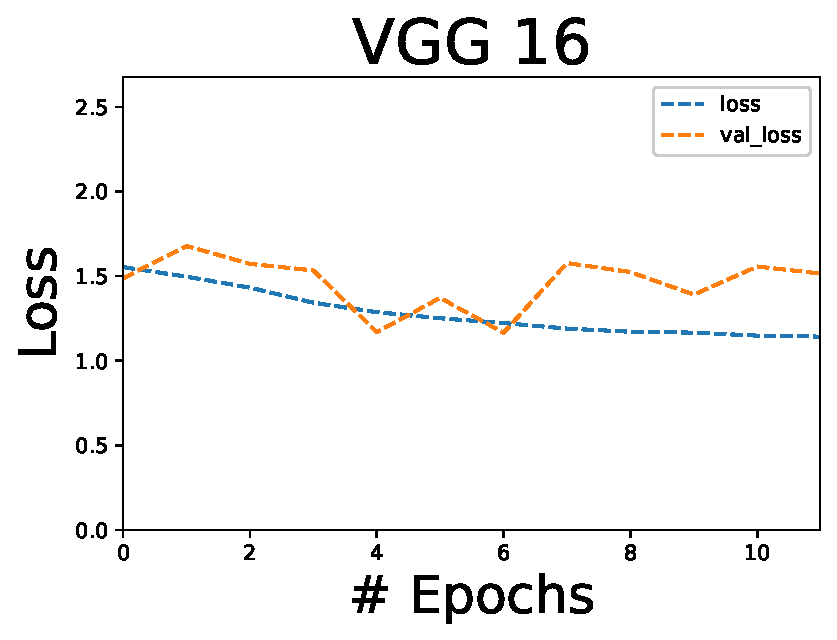
\includegraphics[width=.4\textwidth]{src/images/vgg-regression.eps}
    \caption{Regression loss function of VGG-16 trained on the raw training data set. Although the training loss \path{loss} decreases, the validation loss \path{val_loss} seems to bounce up and down. This model seems to overfit the training data.}
    \label{fig:reg-vgg-loss}
\end{figure}

Due to the fact that the results of MobileNet were somewhat satisfying for the task applied here, no further investigations using other backbones were done.
Generally speaking INet and MobileNet seem to perform similar when trained on the raw data set, while VGG-16 ends up in unsatisfying results for both training sets.
The table (\tabref{fig:two-stage-regression-results}) and the visual components (\figref{fig:regression-samples}) reveal MobileNet as the best performing backbone in combination with an augmented training data set.\\
For the classification task the cropped data set \eqref{eq:cropped-sample} was selected first.
Similar like for regression, this training set was augmented, as well.
The final results can be found in \tabref{fig:classification-results}, which lists the final metrics for the raw training set under "Raw", the augmented ones under "Augmented".
For visual error analysis confusion matrices are used, these confusion matrix can be seen in \figref{fig:classification-inet-conf}, \figref{fig:classification-mobilenet-conf} and \figref{fig:classification-vgg-conf}.
Already for the INet backbone trained on the raw training set it becomes clear that these methods seem to perform better than the previously discussed conventional methods.
A clear diagonal can be seen.
The final, and best, backbone for classification is MobileNet, as the table lists.
The related confusion matrix (\figref{fig:classification-mobilenet-conf}, left) gives arguments for this. The diagonal contains only values $\geq 0.79$ and contains less miss classifications, unlike e.g. INat trained on the augmented training set (\figref{fig:classification-inet-conf}, right).\\
Hence, MobileNet was selected as a backbone for further experiments.\\\newline
To combine two independent CNN architectures, to solve the object detection task, an additional HPO was performed on a training data set that yields samples with the original images \eqref{eq:classification-sample}.
The results of this experiment can as well be found in \tabref{fig:classification-results}, listed as MobileNet with "Uncropped, Raw" in the "Data set" column.
The resulting confusion matrix can be seen in \figref{fig:extra-classification-mobilenet} (left).\\
A last classifier was trained on a training set generated out of the predictions $\mybold{\hat{c}^{(m)}}$ done by the best BB regressor, here MobileNet, trained on the raw train set.
Finally, the 2-stage-models were assembled based on the best models resulting from previously described tests.
\tabref{fig:two-stage-results} contains the results for these experiments.
The final configuration for the independent approach, as well as for the sequential approach is MobileNet as backbone for both models, regression and classification.
\begin{table}[!ht]
    \centering
    \begin{tabular}{|c|c|c|c|c|}
    \hline
        \textbf{Method} & \textbf{GIoU} & \textbf{RMSE} & \textbf{Accuracy} & \textbf{F1}  \\
        \hline
        \textbf{Independent} & $\mybold{0.5602}$ & $\mybold{17.0061}$ & $\mybold{0.8511}$ & $\mybold{0.8462}$\\
        \hline
        Sequential & $0.5602$ & $17.0061$ & $0.5666$ & $0.5661$\\
        \hline
    \end{tabular}
    \caption{Results of experiments with Two-Stage-Methods based on the training set with shapes \eqref{eq:1-stage-sample}. The Regression metrics $\GIoU$ and $\RMSE$ are equal in both cases, because both architectures use the same backbone for regression. Both methods are assembled using MobileNet as backbones for the BB regressor and classifier.}
    \label{fig:two-stage-results}
\end{table}

\subsubsection{Single-Stage-Methods}
For the approach of Single-Stage-Methods, again, three models were assembled, one based on INet, one on MobileNet and one with the VGG-16 as backbone.
The results of the HPOs can be found in \tabref{fig:single-stage-results} (\figref{fig:single-stage-predictions}).
Additional to the HPs from regression and classification, as listed in \tabref{fig:reg-hp-table} and \tabref{fig:clf-hp-table} accordingly, the dropout was configured to be part of the HPO.
For previous HPOs this was omitted because the models, that save tasks individually, seemed to not be impacted by a change in dropout, this was the result of initial experiments, while developing the architectures.
This was not clear from the beginning for the single-stage-methods, hence it was introduced as HP with $d\in[0,1]$ the dropout factor.
The loss weight was set to $\lambda=1$, because it is desired to weight both tasks equally.
Additional to the manually implemented architectures previously mentioned \href{https://github.com/ultralytics/yolov5}{YOLOv5} was trained using the default configurations~\footnote{
    The model was trained based on description from a blog post by Ayoosh Kathuria~\cite{yolo-blog}.
    Further things, such as exporting to TFLite were executed based on descriptions in the code repository (\url{https://github.com/ultralytics/yolov5})
}.
\begin{table}
    \centering
    \begin{tabular}{|c|c|c|c|c|c|}
    \hline
        \textbf{Method} & \textbf{GIoU} & \textbf{RMSE} & \textbf{Accuracy} & \textbf{F1} & \textbf{Inf. time $[s]$} \\
        \hline
        Independent & $0.5638$ &
$17.3479$ & $0.916$ & $0.9168$ & $0.6013$\\
        \hline
        Sequential & $0.5540$ & $18.026241$ & $0.5200$ & $0.5285$ & $0.7869$\\
        \hline
        Single-Stage & $0.3733$
& $19.6725$ & $0.92$ & $0.9197$ & $0.2195$\\
        \hline
        \hline
        \textbf{YOLOv5}
        & $\mybold{0.694285}$
        & $\mybold{18.78450}$
        & $\mybold{0.848}$
        & $\mybold{0.8420}$
        & $\mybold{0.1951}$\\
        \hline
    \end{tabular}
    \caption{Validation test results, based on the test set yielding samples in the shape \eqref{eq:1-stage-sample}, for assembled methods.
    The "Inf. time" value is the average inference time of 5 random samples\footnotemark.}
    \label{fig:final-results}
\end{table}
\footnotetext{These tests have been performed in a private NVIDIA GeForce RTX 2060.}
\subsection{Validation of trained models on the test set}\label{subsec:validation-of-trained-models}
To validate the models the performance was measured using the, in "\nameref{eq:dataset}" mentioned, test set.
These experiments, or tests, are considered representational tests for the models, to see how well they perform on real-life data.
For this purpose the best assembled models from the previous experiments were selected and tested.
The results can be found in the table (\ref{fig:final-results}).
For the independent method the combination MobileNet (regression) trained on the augmented data set and MobileNet (classification) trained on the full images was selected.
The sequential solver contains the same regression model, but uses for classification the MobileNet backbone trained on a training set of predictions $\mybold{c^{(m)}}$ as discussed earlier.
As an additional validation value, the average time of inference in seconds, was calculated for each architecture based on five random selected samples.
Predictions and confusion matrices can be found for two-stage-methods in \tabref{fig:independent-results} (independent), and in \tabref{fig:sequential-results} (sequential).
The related plots for the single-stage-methods can be found in \tabref{fig:single-stage-results}.
Previous training tests allowed the assumption that YOLOv5 outperforms all other methods.
This becomes more visual by looking at sample predictions from YOLO (\ref{fig:yolo-predictions}).
Not only is YOLO capable of performing better, according to metrics (\ref{fig:final-results}), but additionally YOLO is capable of predicting multiple BBs and class labels within the same image (\figref{fig:yolo-predictions}, right).
Compare to all other methods, this is an outstanding improvement.
Hence, it is inevitable to select YOLO for further investigations.
Unfortunately, when comparing the results in \tabref{fig:final-results} with \tabref{fig:classification-results} it becomes evident that something is wrong for the 2-stage independent model, mostly because the accuracy seems to differ a lot.
This should be a target of further investigation, as well.
\begin{figure}[!ht]
    \centering
    \begin{minipage}{.475\textwidth}
        \includegraphics[width=\textwidth]{src/images/val_batch2_labels.png}
    \end{minipage}
    \hfill
    \begin{minipage}{.475\textwidth}
        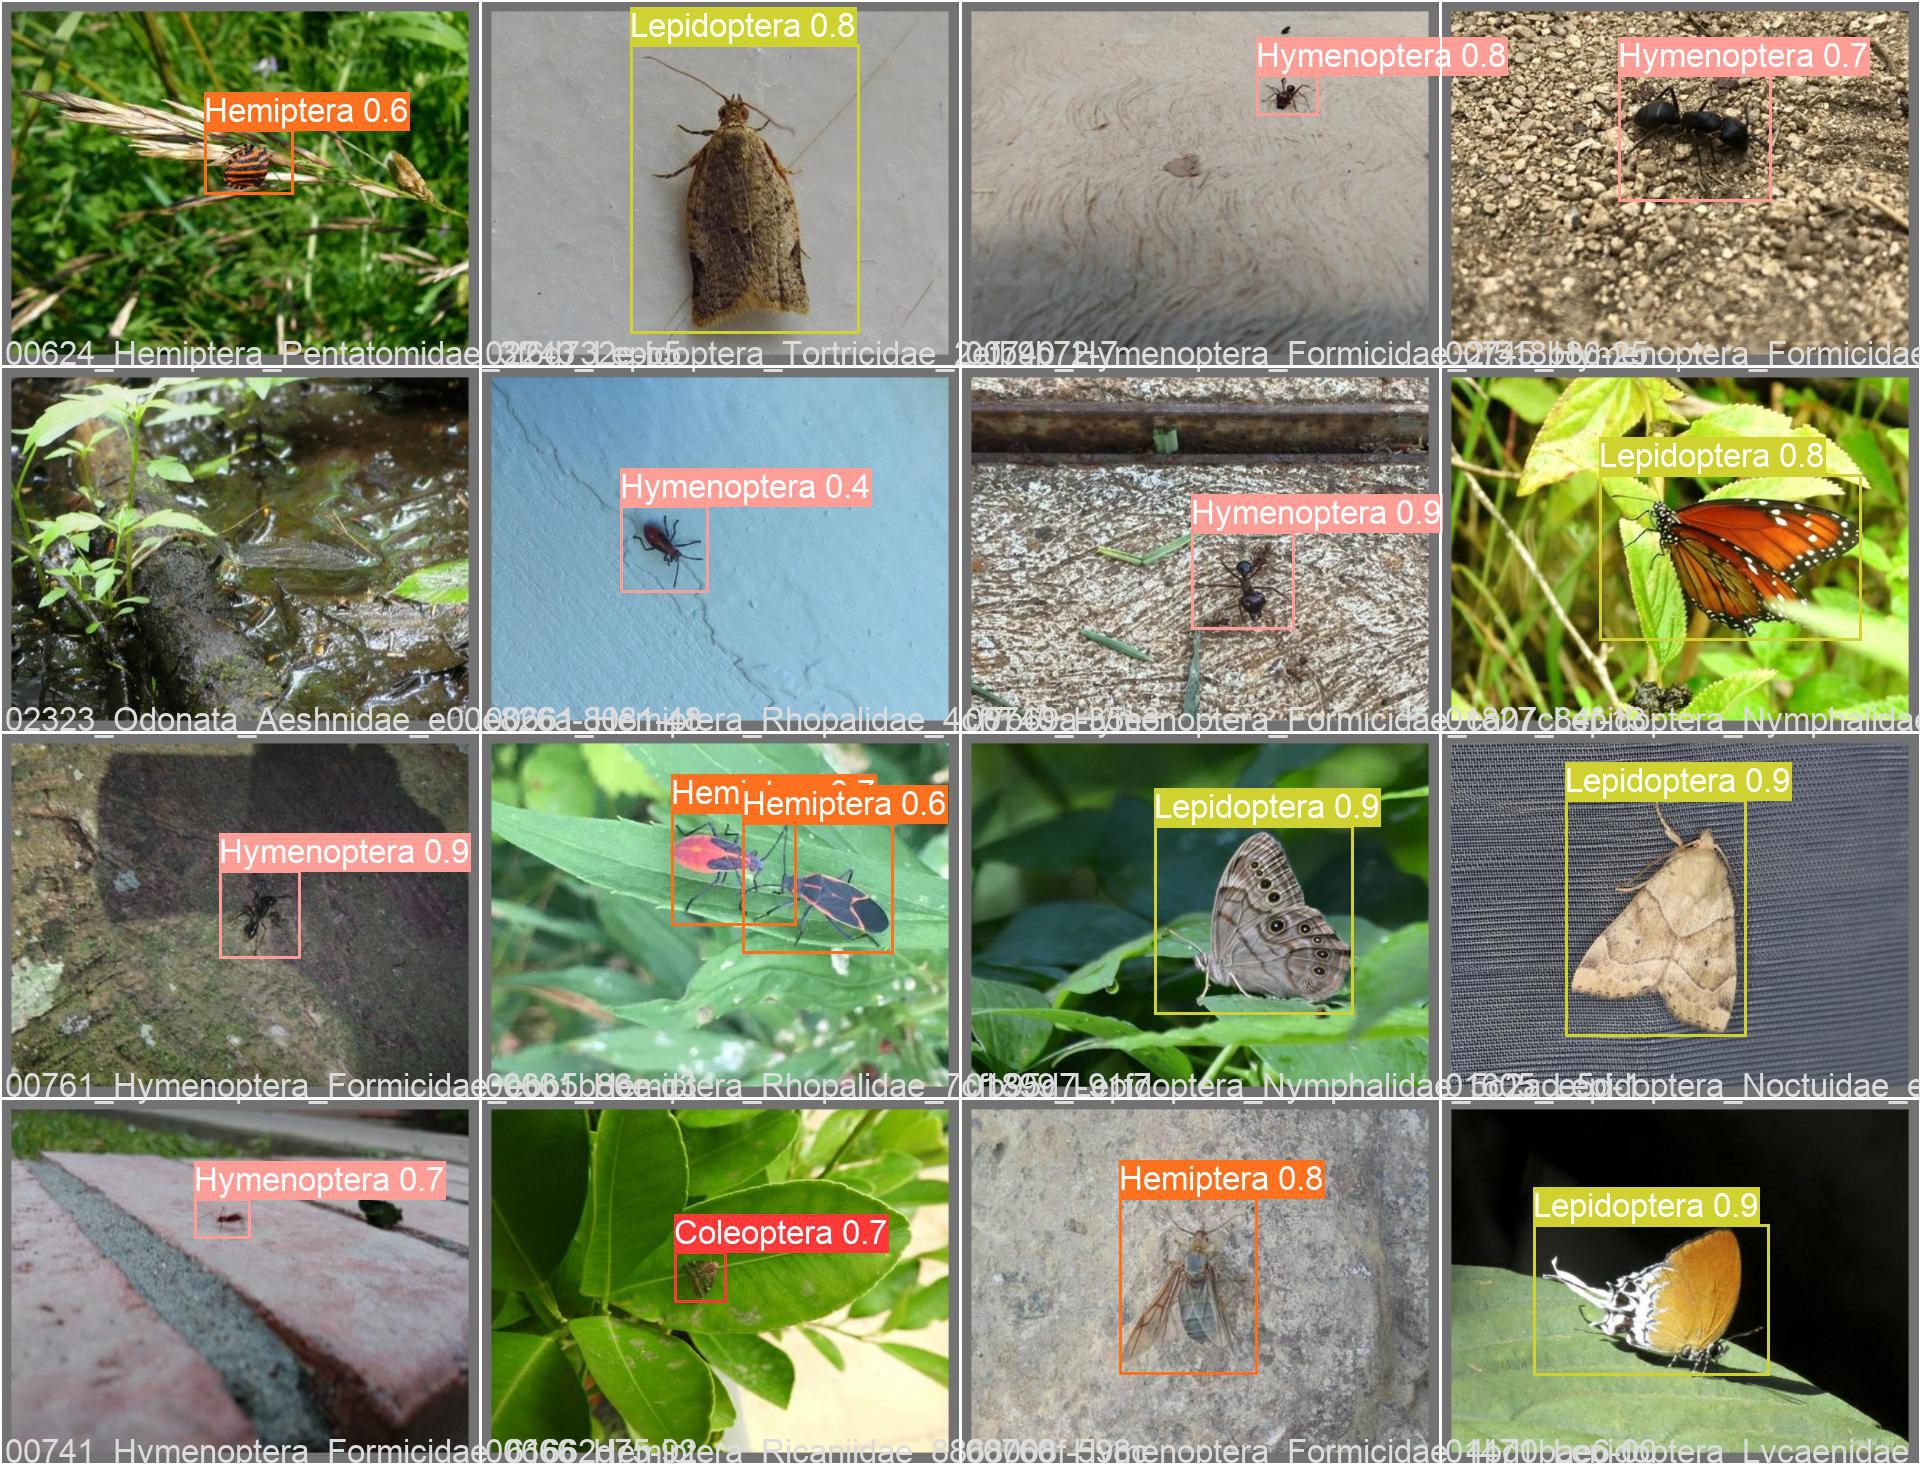
\includegraphics[width=\textwidth]{src/images/val_batch2_pred.png}
    \end{minipage}
    \caption{Predictions performed by YOLOv5. On the left side are single label predictions, here with the BB and label having the highest confidence. The right side contains predictions for one or multiple objects.}
    \label{fig:yolo-predictions}
\end{figure}
\subsection{Hosting on a Raspberry Pi}\label{subsec:hosting-on-raspberry}
This subsection will focus on implementation details which were required to perform to be able to host and use the final models on a RaspberryPi minicomputer.
To reduce the size of a Tensorflow/Keras model several techniques can be applied~\footnote{
    A detailed guide can be found in the \href{https://www.tensorflow.org/model_optimization/guide/get_started}{Tensorflow documentation}.
}.
\subsubsection{Weight Pruning}\label{subsub:weight-pruning}
Weight pruning gradually zeros out model weights during the training process to achieve model sparcity.
Sparse models are easier to compress, and can skip the zeros during inference for latency improvements~\footnote{TF reference: \url{https://www.tensorflow.org/model_optimization/guide/pruning}}.
\subsubsection{Quantization aware training}\label{subsub:quant-aware-training}
Quantization aware training emulates inference-time quantization, creating a model that downstream tools will use to produce actually quantized models. The quantized models use lower-precision (e.g. 8-bit instead of 32-bit float), leading to benefits during deployment~\footnote{TF reference: \url{https://www.tensorflow.org/model_optimization/guide/quantization/training}}.
\subsubsection{Post training Quantization}\label{subsub:quantization}
Post training quantization is another conversion technique that can reduce model size while also improving CPU latency, with little degradation in accuracy.
It allows to train models using floating point values, then convert those weights into TensorFlow Lite format.~\footnote{TF reference: \url{https://www.tensorflow.org/model_optimization/guide/quantization/post_training}}
\subsubsection{Weight Clustering}\label{subsub:weight-clustering}
Weight clustering is a reduction technique that reduces the number of unique weight values in a model.
It first groups the weights of each layer into $N$ clusters, then shares the cluster's centroid value for all the weights belonging to the cluster~\footnote{TF reference: \url{https://www.tensorflow.org/model_optimization/guide/clustering}}.\\\newline
Each of these methods can be applied separately or in combination.
The models assembled for this paper were, as previously mentioned, trained on a server with a "NVIDIA Quadro RTX 8000" GPU and the target is to preserve the calculated weights as far as possible.
Hence, quantization aware training (\ref{subsub:quant-aware-training}) can not be applied.
In the experiments it turned out that the performance of BB regression decreased drastically if a method other than weight clustering is applied.
This is potentially caused by the fact that e.g. Quantization~(\ref{subsub:quantization}) that converts weights from \path{float32} into \path{int8} which trades off precision for size.
The final configuration can be seen in \tabref{fig:reduction}.\\
Visual representations of predictions and confusion matrices can be seen in \figref{fig:tflite-independent-results} (two-stage, independent), \figref{fig:tflite-sequential-results} (two-stage, sequential) and \figref{fig:tflite-single-stage-results} (single-stage).

\begin{table}[!ht]
    \centering
    \begin{tabular}{|l|l|l|l|}
        \hline
        \textbf{Architecture} & \textbf{Method} & \textbf{Initial file size} & \textbf{Final file size} \\
        \hline
        \begin{tabular}{@{}l@{}}
            \textbf{Two-Stage} \\
            \textit{Independent}\\
                Regressor \\
                Classifier \\
        \end{tabular} &
        \begin{tabular}{@{}l@{}}
            \\\\
            (\ref{subsub:weight-clustering}.) \\
            (\ref{subsub:quantization}.) \\
        \end{tabular} &
        \begin{tabular}{@{}l@{}}
            \\\\
            40,6 MB \\
            40,6 MB \\
        \end{tabular}&
        \begin{tabular}{@{}l@{}}
            \\\\
            \;3,6 MB \\
            13,3 MB \\
        \end{tabular}
        \\ % end first line
        \hline
        \begin{tabular}{@{}l@{}}
            \textit{Sequential}\\
                Regressor \\
                Classifier \\
        \end{tabular} &
        \begin{tabular}{@{}l@{}}
            \\
            (\ref{subsub:weight-clustering}.) \\
            (\ref{subsub:quantization}.) \\
        \end{tabular} &
        \begin{tabular}{@{}l@{}}
            \\
            40,6 MB \\
            14,8 MB \\
        \end{tabular}&
        \begin{tabular}{@{}l@{}}
            \\
            13,3 MB \\
            \;3,6 MB \\
        \end{tabular}
        \\
        \hline
        \begin{tabular}{@{}l@{}}
            \textbf{Single-Stage} \\
                Model \\
                YOLOv5
        \end{tabular} &
        \begin{tabular}{@{}l@{}}
            \\
            (\ref{subsub:weight-clustering}.) \\
            -
        \end{tabular} &
        \begin{tabular}{@{}l@{}}
            \\
            42,2 MB \\
            13.7 MB
        \end{tabular}&
        \begin{tabular}{@{}l@{}}
            \\
            13.9 MB \\
            14.2 MB
        \end{tabular}
        \\
        \hline
    \end{tabular}
    \caption{Executed model optimization for architectures to allow faster inference on a Raspberry Pi. Whilst own implementations seem to decrease drastically in size, especially the classifiers, YOLOv5 reduces its size by only a bit more than 1 MB.}
    \label{fig:reduction}
\end{table}
The optimization method for YOLOv5 is the interal configuration from the code repository that are available through one of the accommodating scripts, called \path{export.py}.\\\newline
After converting the models into TF Lite format, the previously described \hyperref[subsec:validation-of-trained-models]{validation tests} were performed again on, this time on a Raspberry Pi using the reduced model weights.
The results of these tests can be found in \tabref{fig:final-results-tflite}.
Again, YOLOv5 outperforms the remaining methods.
But it comes with a big trade-off.
Whilst the predictive performance is great, the inference time increases by a factor if $10$, compared to the custom single-stage method.
This speed decrease is caused by the validation process of YOLO, that validates the set of many BB proposals extracted by the model, to then return the most promising prediction.\\
Under the restriction to only use one of the models implemented and analyzed thoroughly, by this paper, the decision for the final model would be using the independent method.
Not only the sequential method performs worse for the regression task, also the inference time increased is lower.
This is most likely due to the fact that the independent method does not need to crop the image, prior to classification.
The speed decrease, compared to the single-stage method, is drastic, by a factor of $3$ and might be due to the fact that the independent method is processing the image twice, instead of once like the single-stage method.
Over all, it seems that the classification task is easier to solve for the here analyzed CNN architectures.
\begin{table}
    \centering
    \begin{tabular}{|c|c|c|c|c|c|}
    \hline
        \textbf{Method} & \textbf{GIoU} & \textbf{RMSE} & \textbf{Accuracy} & \textbf{F1} & \textbf{Inf. time $[s]$} \\
        \hline
        Independent & $0.5540$ &
$18.02641$ & $0.9200$ & $0.9210$ & $1.3140$\\
        \hline
        Sequential & $0.5540$ & $18.0262$ & $0.5200$ & $0.5285$ & $2.2799$\\
        \hline
        Single-Stage & $0.1833$
& $21.7866$ & $0.6080$ & $0.5804$ & $0.7272$\\
        \hline
        \hline
        \textbf{YOLOv5} & $\mybold{0.6847}$ & $\mybold{22.7424}$ & $\mybold{0.82}$ & $\mybold{0.8091}$ & $\mybold{2.084}$\\
        \hline
    \end{tabular}
    \caption{Test results for final TF Lite versions, based on the test set that yields objects in shape \eqref{eq:1-stage-sample}.
    }
    \label{fig:final-results-tflite}
\end{table}

\subsection{Roadblocks}\label{subsec:roadblocks}
The following section will give a brief overview of main problems faced while working on this project to allow the reader to learn from mistakes done along the road.
\subsubsection{Data sets and Augmentation}
The here used data sets are highly influenced by the \lstinline{Dataset} class provided in the \href{https://www.tensorflow.org/api_docs/python/tf/data/Dataset}{Tensorflow API} and are built using the \href{https://www.tensorflow.org/api_docs/python/tf/data/Dataset#from_generator}{generator} approach.
Data sets generated using generators are iterable, sequential data sets that allow lazy loading of the underlying samples.
Instead of preallocating the full amount of memory required for the data set it loads elements on demand.
This can either be single samples or batches of samples.
For the purpose of \textbf{two-stage-models} and \textbf{single-stage-models} a total of three data set preperation helpers were created.
One for the Regression task, one for the Classification task and one data set that contains combined outputs.
To follow the generator idiom the here implemented data augmentation pipeline works in a similar way.
Instead of storing all augmented samples in advance, to then load samples during training, the \lstinline[language=Python]{DataAugmentationHelper} class wraps around the data set and creates a new generator data set that yields augmented samples.
This allows simple replacement of augmentation methods in the helper class.
And also reduces resource requirements in the training phase of the, mostly, magnitudes bigger augmented data set.
\subsubsection{GIoU-Loss}
One of the major obstacles to overcome was understanding Tensorflow-AddOn's implementation~\footnote{Tensorflow-AddOn's documentation for GIoULoss: \url{https://www.tensorflow.org/addons/api_docs/python/tfa/losses/GIoULoss}} of the GIoU-Loss.
Initially a convention of
\begin{align*}
    \mybold{c^{(m)}} = \left(x^{(m)}_{\min}, y^{(m)}_{\min}, x^{(m)}_{\max}, y^{(m)}_{\max}\right)
\end{align*}
for the BB coordinate labels was used to apply the supervised learning technique.
This turned out to make the CNN architectures converge to solutions in which the model predicts BBs with either height or width component equal to zero.
To solve this, the previously introduced format of $\mybold{c^{(m)}} = \left(y^{(m)}_{\min}, x^{(m)}_{\min}, h^{(m)}, w^{(m)}\right)^T$\eqref{eq:bb} was used to enforce learning of the aspect ratios of the BB rather than two independent coordinates.
Unfortunately Tensorflows implementation of \lstinline{GIoU} uses the format $\mybold{c^{(m)}} = \left(y^{(m)}_{\min}, x^{(m)}_{\min}, y^{(m)}_{\max}, x^{(m)}_{\max}\right)^T$ hence a wrapper~\footnote{This wrapper can be found in \path{src/losses/giou_loss.py}} was built for the conversion
\begin{align*}
    \left(y^{(m)}_{\min}, x^{(m)}_{\min}, h^{(m)}, w^{(m)}\right)^T \rightarrow \left(y^{(m)}_{\min}, x^{(m)}_{\min}, y^{(m)}_{\max}, x^{(m)}_{\max}\right)^T\quad .
\end{align*}
\subsubsection{Tensorflow 2.4 vs. Tensorflow 2.8}
The accommodating code repository was developed on a machine running Tensorflow v2.8, without the option of down-grading to a version prior to 2.6, but tests and experiments were executed on a machine running Tensorflow v2.4.
This caused a big headache while implementing several building blocks for this paper, such as all of the dedicated Model classes in \path{src/models} and data sets in \path{src/data}.
Thankfully the developers of Tensorflow maintain backward compatibility between package versions, which allows usage of code developed under 2.4 to run under version 2.6.
Hence, after back-porting the code it was ensured to be executable under the newer version.
\subsubsection{Dedicated Object Detection Architectures}
Apart from CNNs, that are introduced in this paper, more complex architectures such as YOLO~\cite{yolo}, or MobileNet-SSD~\cite{MobileNet} were presented over the last decades, these architectures seem to perform very well on object detection tasks.
Due to their complexity in their architecture it was not possible considering the time constraints of this paper, to test fine-tuning or training these architectures.
The likelihood is very high that these architectures solve the task better, and I would suggest the reader and my successor at \textit{KInsecta} to look into them and compare results with the benchmarks presented here.
Unfortunately, due to hardware and time constraints, it was not possible to display results of the originally trained model further. This is due to the fact that YOLOv5 is implemented in PyTorch rather than Tensorflow.
